% \documentclass[aspectratio=169]{beamer} % 16:9
\documentclass{beamer}
\usepackage{ctex, hyperref}
\usepackage[T1]{fontenc}
\graphicspath{{pic/}}

% other packages
\usepackage{latexsym, amsmath, xcolor, multicol,booktabs, calligra}
\usepackage{graphicx, pstricks, listings, stackengine}

\author[Sunbowen Lee]{李孙博闻}
\title[Graph neural network]{图神经网络的温和入门}
% \subtitle{图神经网络介绍}
\institute{武汉科技大学 \\ 理学院 \\ 冶金工业过程系统科学湖北省重点实验室}
\date{\today}
\usepackage{wust}

% 定义颜色
\def\cmd#1{\texttt{\color{red}\footnotesize $\backslash$#1}}
\def\env#1{\texttt{\color{blue}\footnotesize #1}}
\definecolor{deepblue}{rgb}{0,0,0.5}
\definecolor{deepred}{rgb}{0.6,0,0}
\definecolor{deepgreen}{rgb}{0.05, 0.44, 0.29}  % 青山绿
\definecolor{lightblue}{rgb}{0.63, 0.80, 0.86}  % 沁湖蓝

\lstset{
    basicstyle=\ttfamily\small,
    keywordstyle=\bfseries\color{deepblue},
    emphstyle=\ttfamily\color{deepred},    % Custom highlighting style
    stringstyle=\color{deepgreen},
    numbers=left,
    numberstyle=\small\color{halfgray},
    rulesepcolor=\color{red!20!green!20!blue!20},
    frame=shadowbox,
}

\begin{document}

\kaishu
\begin{frame}  % 封面
    \titlepage
    \begin{figure}[htpb]
        \centering
        \vspace{-0.7cm}
        
\includegraphics[width=0.45\linewidth]{wust.png}
    \end{figure}
\end{frame}

\begin{frame}{前言}
    尽管图网络具体实现可通过简单调包实现,但在此之前仍然需要了解图的基础知识,掌握``图嵌入''的概念,即如何把数据整理为图网络可以计算的嵌入向量形式,然后才能正确调包。\newline

    本幻灯片材料主要参考Sanchez-Lengeling\cite{sanchez-lengeling2021a}等人的论文.
\end{frame}

\begin{frame}{目录}
    %\begin{multicols}{2}
        \tableofcontents[sectionstyle=show,subsectionstyle=hide]
    %\end{multicols}
\end{frame}


\section{图结构基础}

% \begin{itemize} % [<+-| alert@+>]

\begin{frame}{Vertex, Edge and Global}
    \begin{figure}
        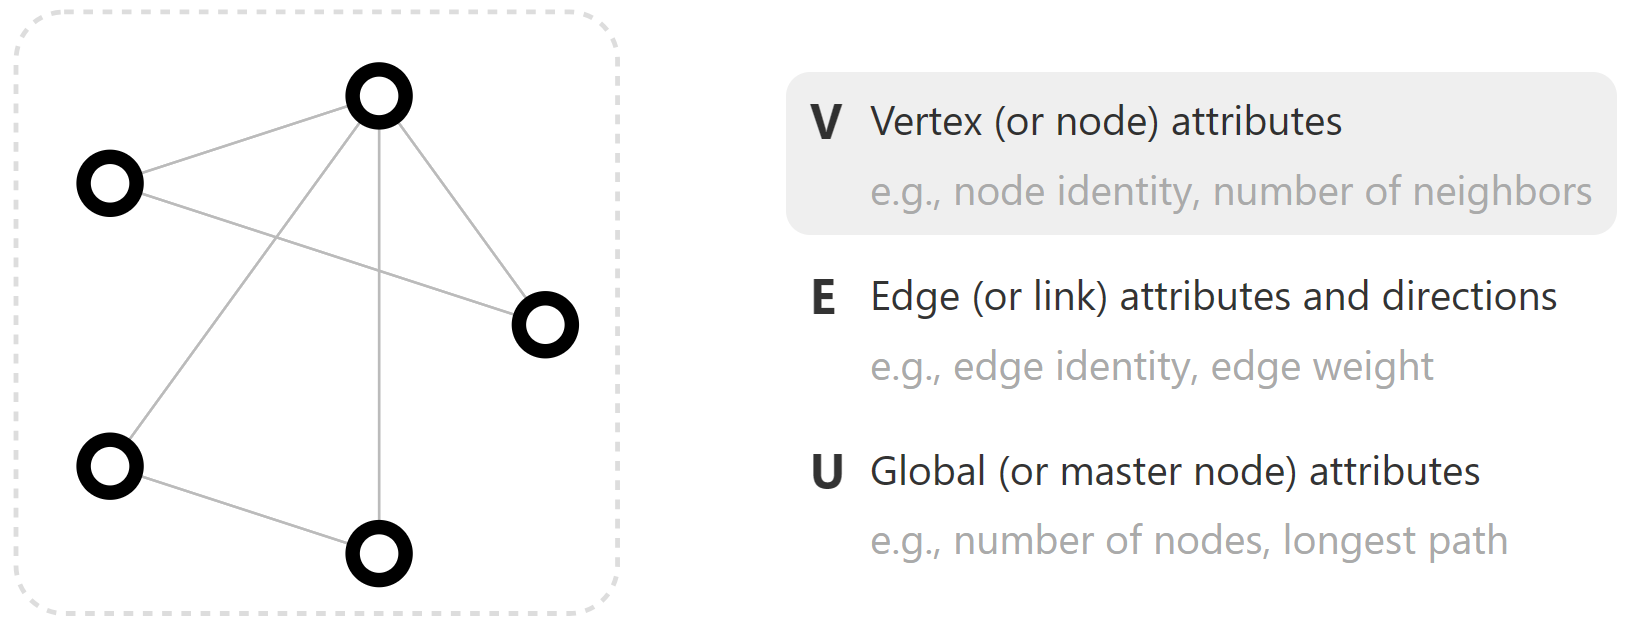
\includegraphics[width=\textwidth]{vertex.png}
    \end{figure}
\end{frame}

\begin{frame}{Vertex, Edge and Global}
    \begin{figure}
        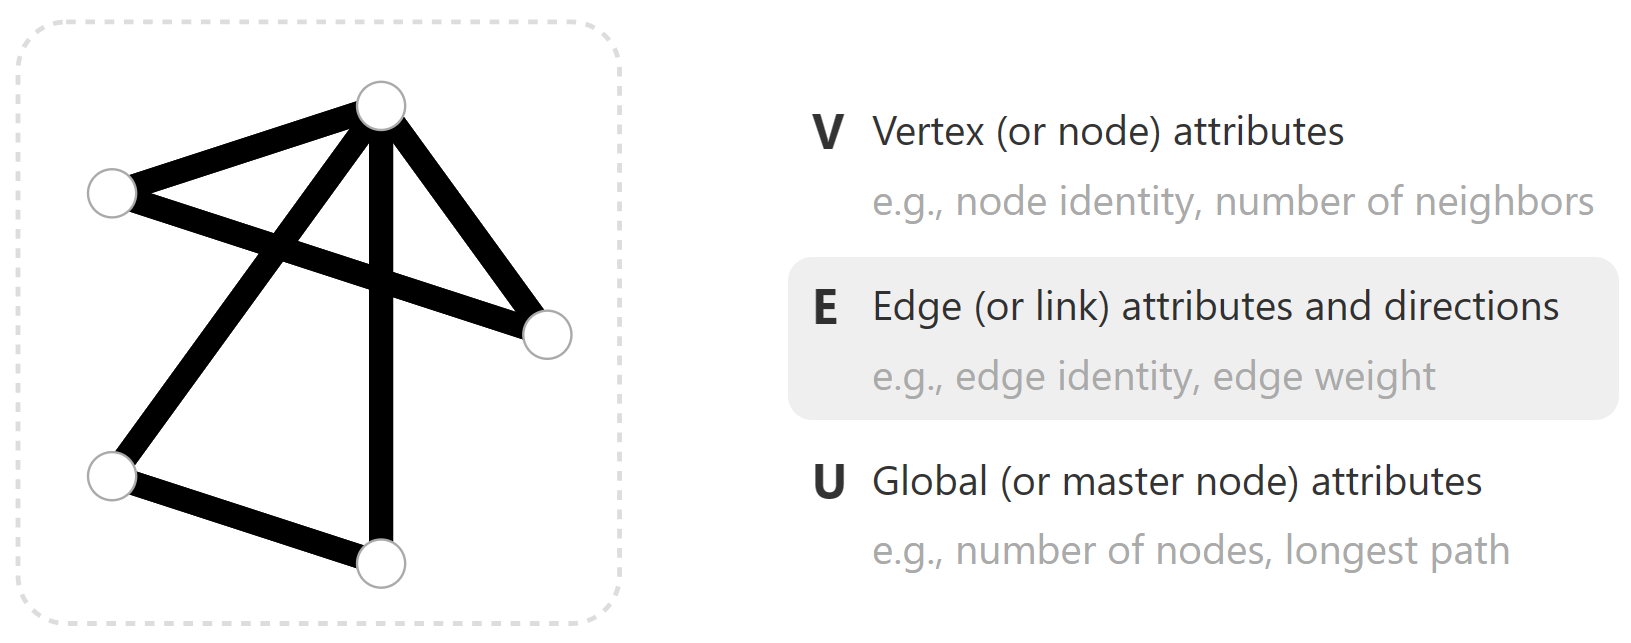
\includegraphics[width=\textwidth]{edge.png}
    \end{figure}
\end{frame}

\begin{frame}{Vertex, Edge and Global}
    \begin{figure}
        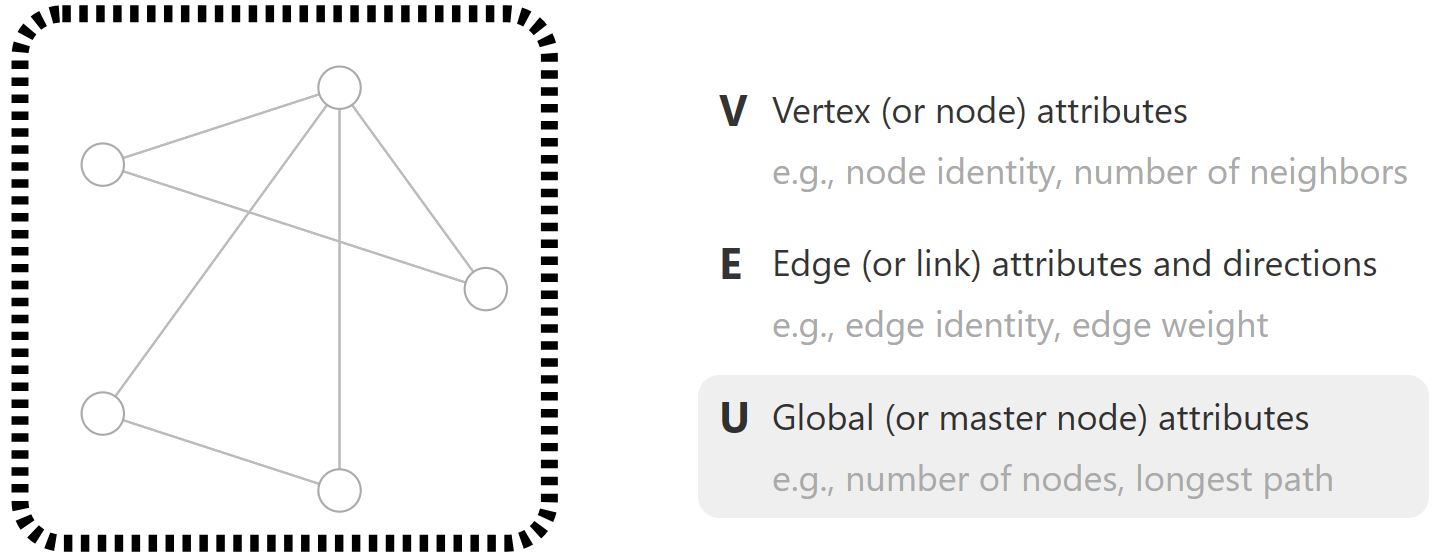
\includegraphics[width=\textwidth]{global.png}
    \end{figure}
    注意全局用U而非G表示。
\end{frame}

\begin{frame}{Vertex, Edge and Global}
    \begin{figure}
        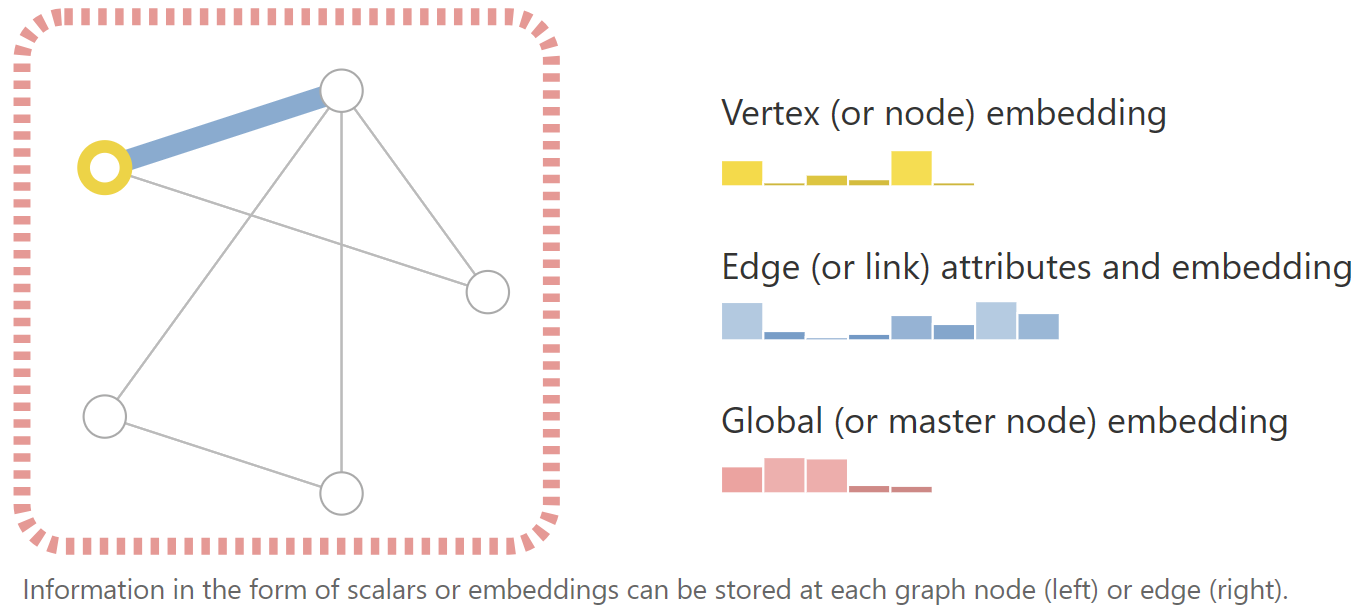
\includegraphics[width=\textwidth]{graph.png}
    \end{figure}
    图的三种元素都可以包含嵌入向量,这里嵌入是一维的,可视化呈现。
\end{frame}

\section{哪里有图结构?}

\begin{frame}{从图像到图}
    \begin{figure}
        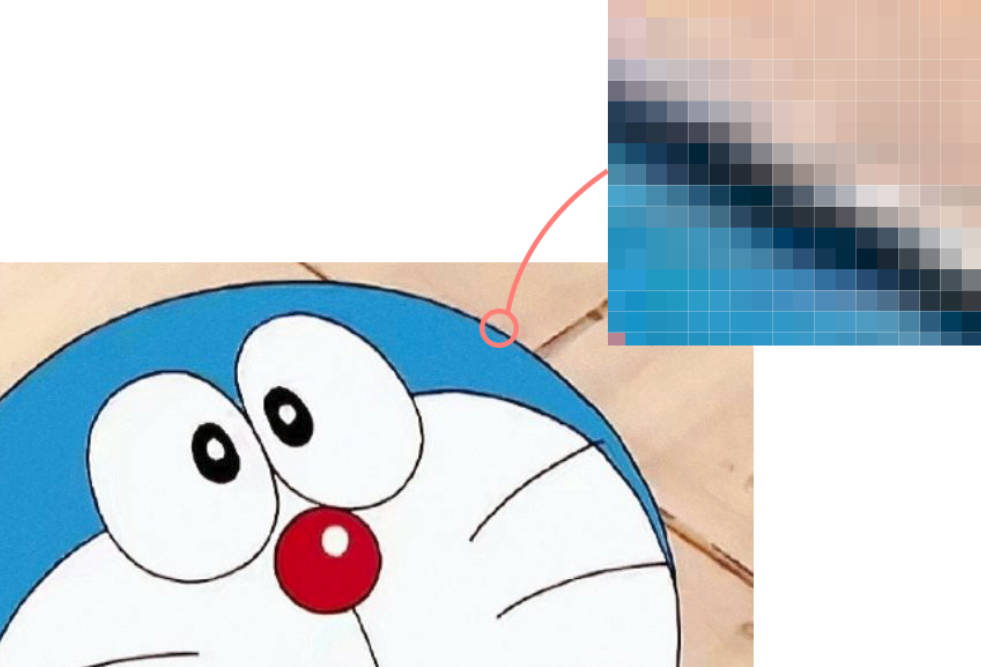
\includegraphics[width=0.5\textwidth]{图片像素.jpg}
        \caption{图片是由许多像素点构成的,每个像素点有一个或多个数值,如灰度值或者RGB值。}
    \end{figure}
\end{frame}

\begin{frame}{从图像到图}
    \begin{figure}
        \includegraphics[width=\textwidth]{图1.jpg}
        \caption{左边是图像,中间是邻接矩阵,右边是图。}
    \end{figure}
    图像也可以表示为图,一个5*5的图像可以表示为邻接矩阵和图的形式。这里三种不同的表现方法是同一个信息的不同表示方法。
\end{frame}

\begin{frame}{句子表示为图}
    \begin{figure}
        \includegraphics[width=\textwidth]{图2.jpg}
        \caption{语句表现为图的形式。}
    \end{figure}
    这里邻接矩阵去掉了对角连接和下三角表示。另外,语句在机器学习中通常不会用图表示,而是通过编码并映射到嵌入向量。
\end{frame}

\begin{frame}{分子图}
    \begin{figure}
        \includegraphics[width=\textwidth]{图3.jpg}
        \caption{分子结构表现为图。}
    \end{figure}
    相比于前面的图,分子图更具有异质性。
\end{frame}

\begin{frame}{人物关系图}
    \begin{figure}
        \includegraphics[width=\textwidth]{图4.jpg}
        \caption{人物关系建模为图。}
    \end{figure}
    话剧奥赛罗中的人物关系可以建模为图,节点表现为角色,边建模为人物间联系。
\end{frame}

\begin{frame}{论文关系图}
    \begin{figure}
        \includegraphics[width=0.5\textwidth]{图5.jpg}
        \caption{文章引用表示为图}
    \end{figure}
\end{frame}

\section{图任务}

\begin{frame}{图分类任务}
    \begin{figure}
        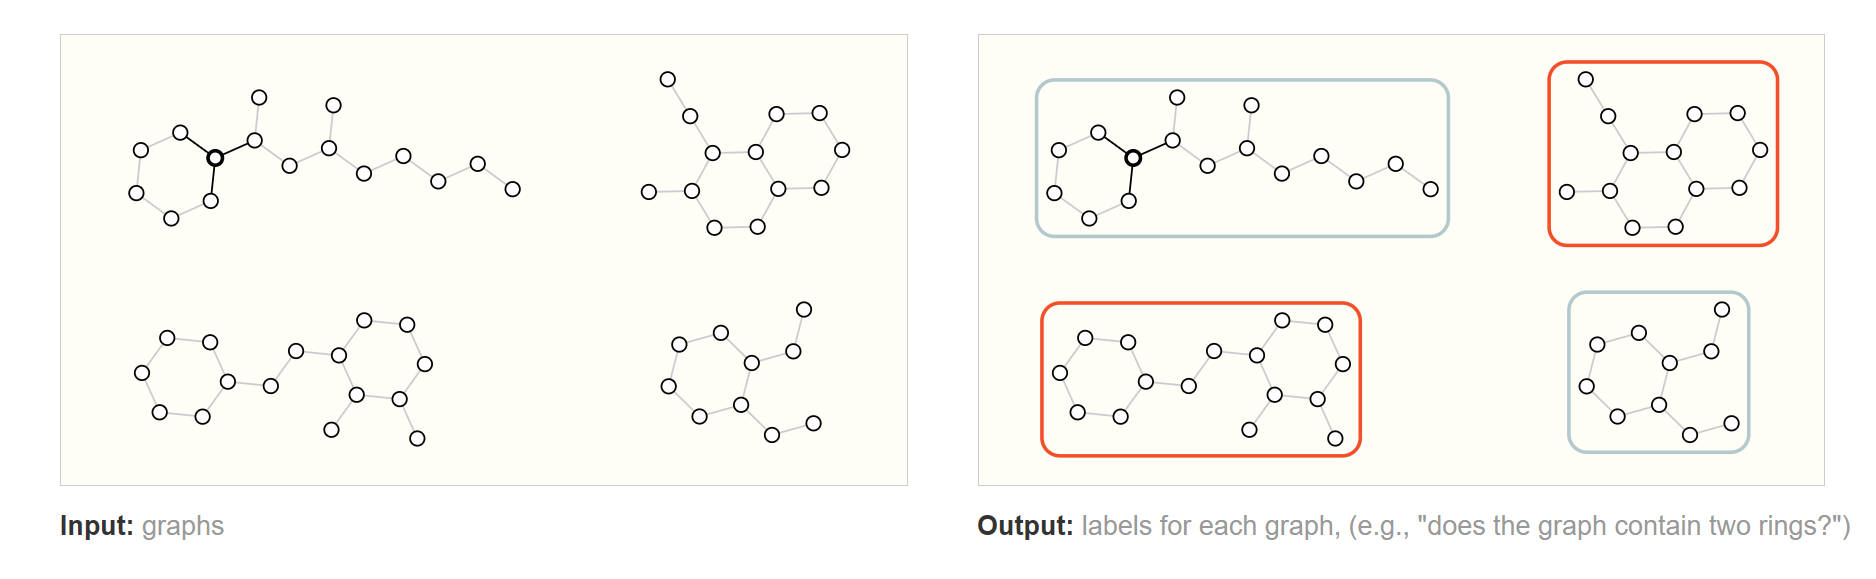
\includegraphics[width=\textwidth]{全局分类.jpg}
        \caption{识别哪些分子有两个苯环}
    \end{figure}
    输入多个分子的图信息,输出各个图的类别。
\end{frame}

\begin{frame}{点分类任务}
    \begin{figure}
        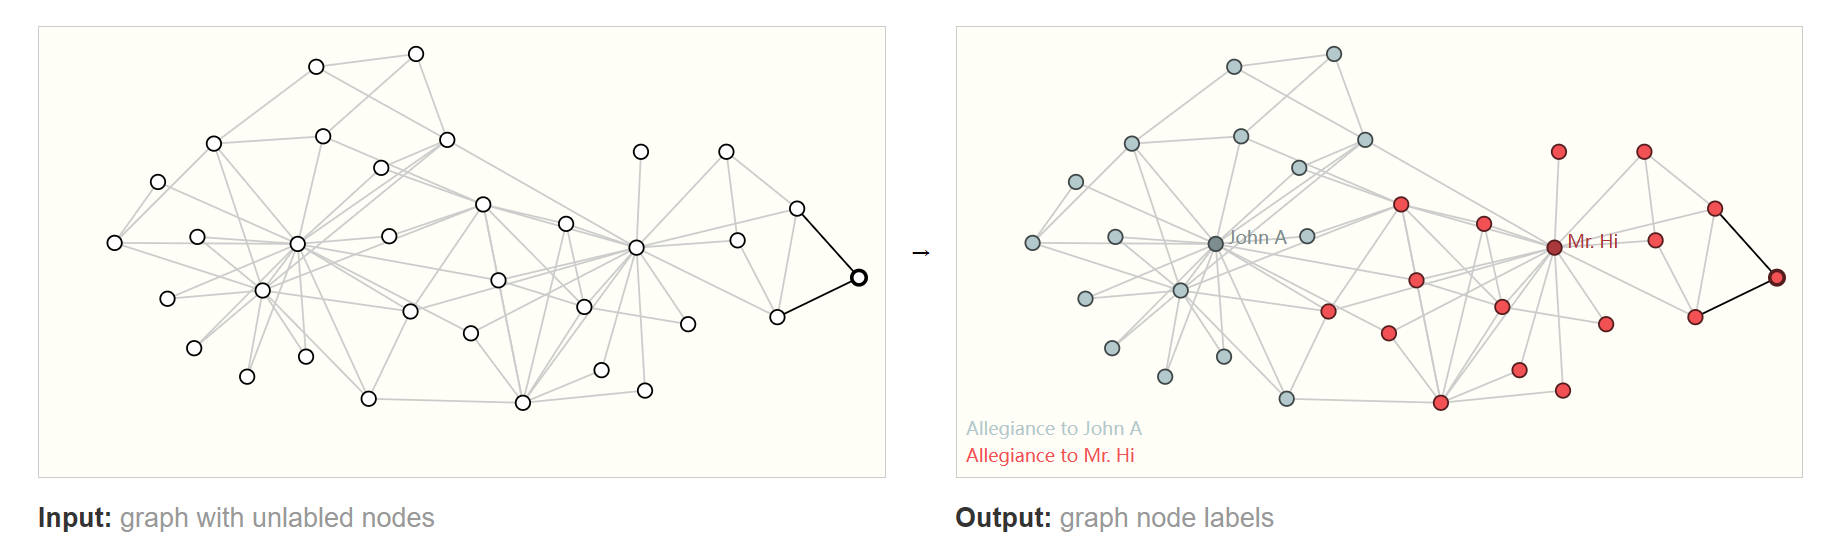
\includegraphics[width=\textwidth]{点分类.jpg}
        \caption{识别那些人支持John H,哪些人支持Hi。}
    \end{figure}
    输入一个图,输出各个点的类别,这里是二分类。
\end{frame}

\begin{frame}{边分类任务}
    \begin{figure}
        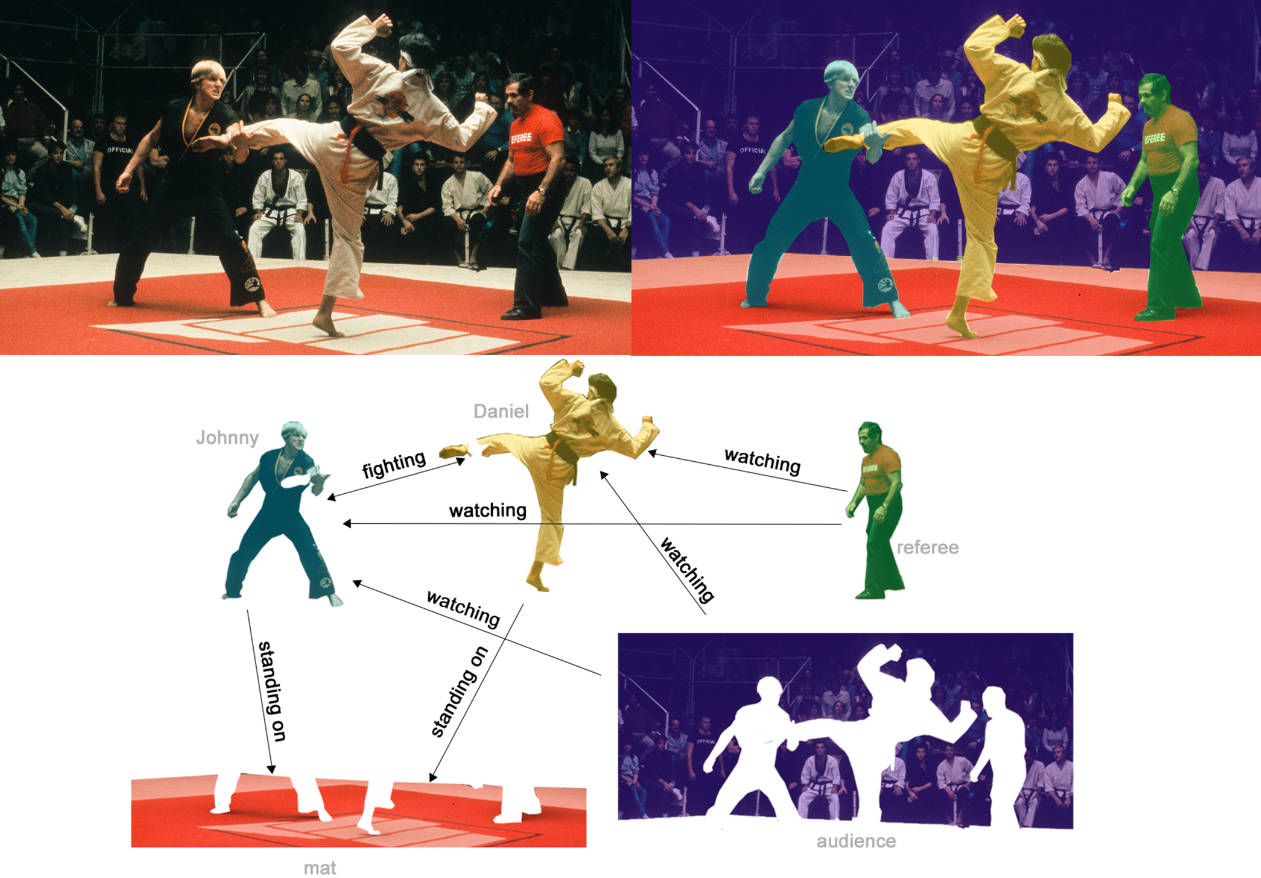
\includegraphics[width=0.7\textwidth]{边分类.jpg}
        \caption{先对图片做分割,然后把被分割的部分作为节点,识别各个节点之间的关系。对局者站在垫子上,对局者相互对抗,裁判和观众观看对抗。}
    \end{figure}
\end{frame}

\begin{frame}{边分类任务}
    \begin{figure}
        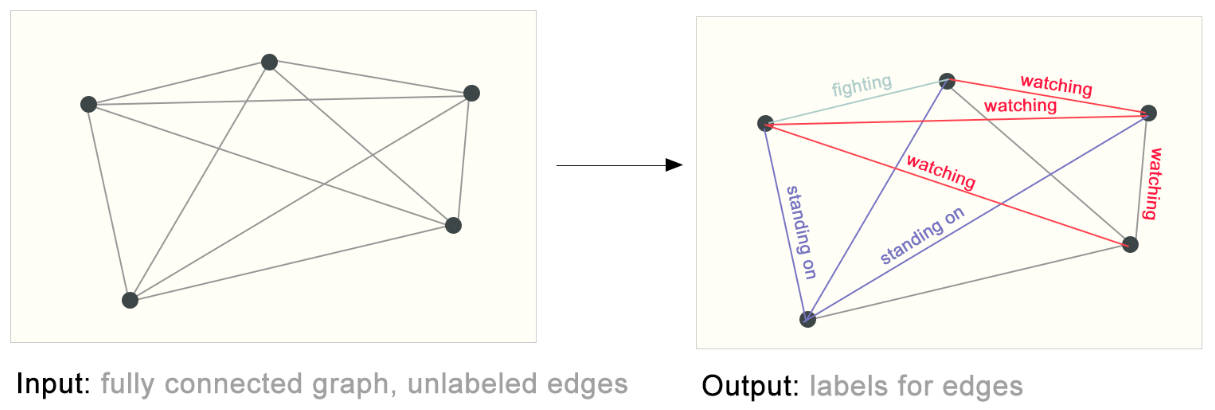
\includegraphics[width=\textwidth]{边分类2.jpg}
        \caption{图 9 简化图。}
    \end{figure}
\end{frame}

\section{图的构建}

\begin{frame}{邻接矩阵不足以表示图}
    \begin{figure}
        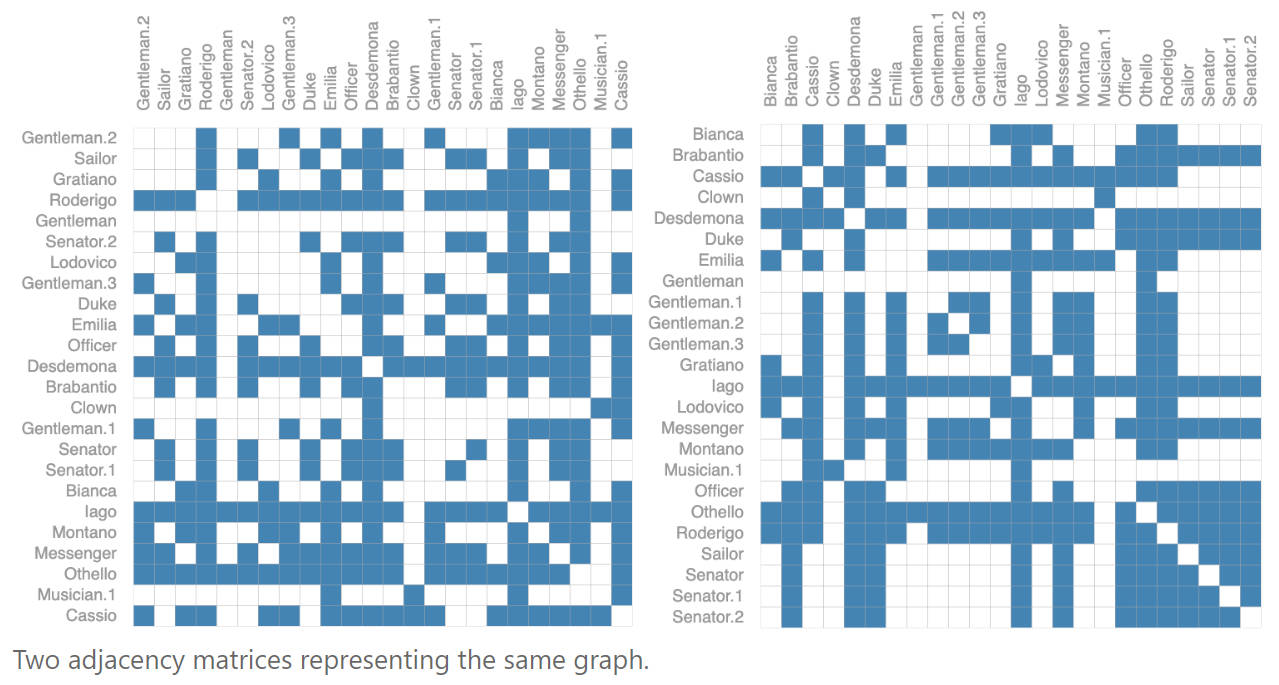
\includegraphics[width=0.9\textwidth]{邻接矩阵.jpg}
        \caption{邻接矩阵经过初等变换,即行变换或者列变换,其含义并没有改变,但是矩阵特征发生很大改变。}
    \end{figure}
\end{frame}

\begin{frame}{图嵌入}
    \begin{figure}
        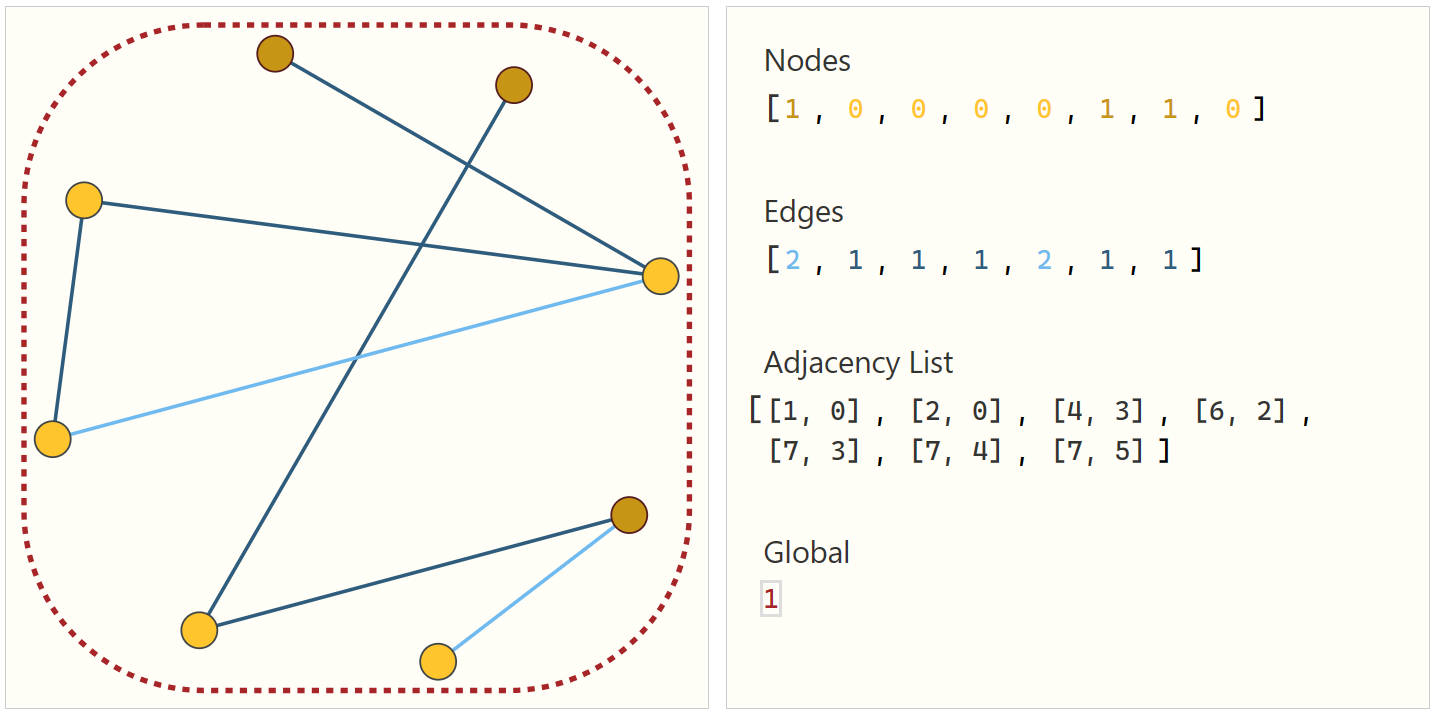
\includegraphics[width=0.9\textwidth]{图嵌入.jpg}
        \caption{邻接矩阵无法用于学习,但是图可以转化为嵌入向量形式以用于学习。三个嵌入向量可以准确表示图信息。}
    \end{figure}
\end{frame}

\begin{frame}{图嵌入}
    \begin{itemize}[<+-| alert@+>]
        \item 以节点举例,图 12 中一个节点可以表示为0和1两个数字,实际上也可以表示为任意维度的张量,其他元素同理。
        \item 如果一个节点表示一个学生,它的节点可以是包含多个信息的向量,比如【性别、班级、学校】。
        \item 这里的邻接表可以表示为其他不同的形式,以使用的图网络的包的要求为准。
    \end{itemize}
\end{frame}

\section{图神经网络}

\begin{frame}

\end{frame}

\section{参考文献}

\begin{frame} %[allowframebreaks]
    \bibliography{ref}
    \bibliographystyle{plain}
    % 如果参考文献太多的话,可以像下面这样调整字体:
    % \tiny\bibliographystyle{alpha}
\end{frame}

\begin{frame}
    \begin{center}
        {\Huge\calligra Thanks!}
    \end{center}
\end{frame}

\end{document}